\documentclass[a4paper,12pt,svgnames]{report}
\usepackage{preamble}

\pagestyle{empty}

\begin{document}
\begin{center}
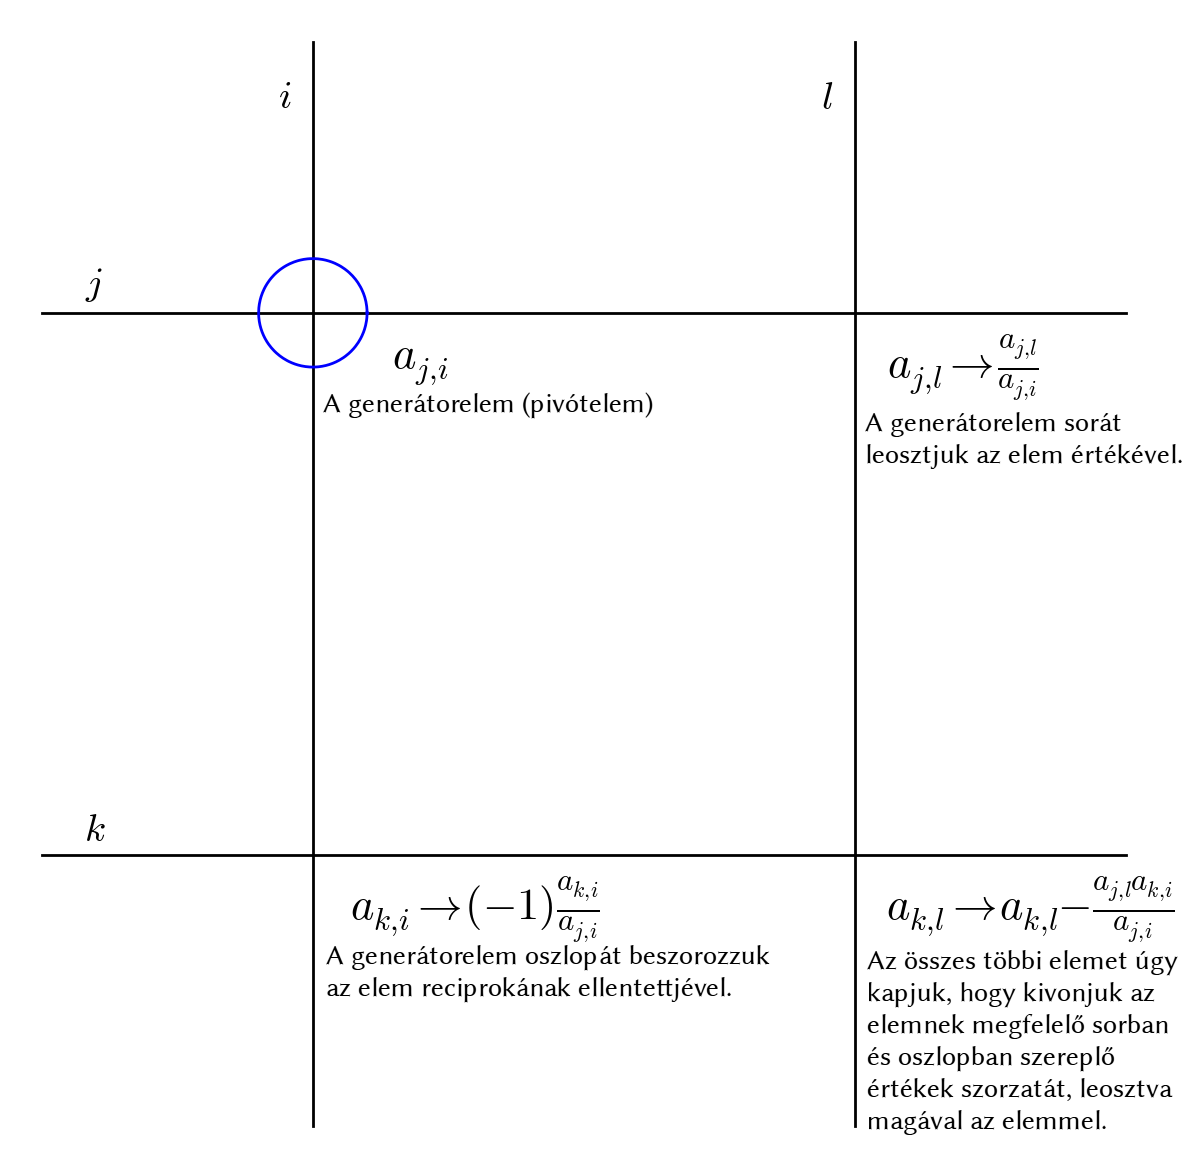
\includegraphics[scale=0.75]{opkut.png}
\end{center}
\medskip\hrule\medskip
\indent Egy üzem kétféle terméket gyárt ($T_1$,$T_2$). A termékek három alkatrész ($A_1$,$A_2$,$A_3$) felhasználásával készülnek. Az első táblázat a termékek szerelési idejét, egységárát és az alkatrészigényüket tartalmazza. Az alkatrészek megmunkálását két gépen végzik ($G_1$,$G_2$). A második táblázat az alkatrészek gépenkénti megmunkálási igényét tartalmazza, és a megmunkálógépek kapacitását. A szerelőüzem kapacitása 220 perc/nap. Határozza meg a szerelő- és gyártóüzem kapacitását nem meghaladó napi termelést úgy, hogy az árbevétel maximális legyen!
\begin{align*}
\begin{tabular}{c|ccc|c|c|}
\multicolumn{1}{c}{}&\multicolumn{1}{c}{$A_1$}&\multicolumn{1}{c}{$A_2$}&
\multicolumn{1}{c}{$A_3$}&\multicolumn{1}{c}{Szerelés}&
\multicolumn{1}{c}{Egységár}\\\cline{2-6}
$G_1$&$1$&$0$&$2$&$2$&$27$\\
$G_2$&$0$&$1$&$1$&$1$&$8$\\\cline{2-6}
\end{tabular}&&
\begin{tabular}{c|ccc|c|}
\multicolumn{1}{c}{}&\multicolumn{1}{c}{$A_1$}&\multicolumn{1}{c}{$A_2$}&
\multicolumn{1}{c}{$A_3$}&\multicolumn{1}{c}{Kapacitás}\\\cline{2-5}
$G_1$&$1$&$0$&$1$&$240$\\
$G_2$&$7$&$1$&$1$&$630$\\\cline{2-5}
\end{tabular}
\end{align*}

Először is a megoldáshoz fel kell írnunk a matematikai modellt, amelyhez ki kell hámoznunk az adatokat a táblázatokból:
\begin{alignat*}{6}
1\cdot 1x_1&+&0\cdot0x_2&+&1\cdot2x_3&+&1\cdot0x_1&+&0\cdot1x_2&+&1\cdot1x_3&\leq240\\
7\cdot1x_1&+&1\cdot0x_2&+&1\cdot2x_3&+&7\cdot0x_1&+&1\cdot1x_2&+&1\cdot1x_3&\leq630\\
&&&&&&&&2x_1&+&1x_2&\leq220\\
&&&\mathrlap{27x_1+8x_2\longrightarrow\max!}
\end{alignat*}

azaz
\begin{alignat*}{3}
3x_1&+&x_2&\leq240\\
9x_1&+&2x_2&\leq630\\
2x_1&+&1x_2&\leq220\\
27x_1&+&8x_2&\longrightarrow\max!\\
x_1&,&x_2&\geq0
\end{alignat*}

A következő lépés az LP feladat sztenderdizálása:
\begin{alignat*}{5}
3x_1&+&x_2&+&s_1&=240\\
9x_1&+&2x_2&+&s_2&=630\\
2x_1&+&1x_2&+&s_3&=220\\
&&\mathclap{27x_1+8x_2\longrightarrow\max!}\\
&&&&&&\mathllap{x_1,x_2,s_1,s_2,s_3\geq0}
\end{alignat*}

\begin{multicols}{2}
\begin{tabular}{c|cc|c|}
\multicolumn{1}{c}{}&\multicolumn{1}{c}{$x_1$}&
\multicolumn{1}{c}{$x_2$}&\multicolumn{1}{c}{}\\\cline{2-4}
$s_1$&  $2$& \circled{$1$}& $220$\\
$s_2$&  $3$& $1$& $240$\\
$s_3$&  $9$& $2$& $630$\\\cline{2-4}
     & $27$& $8$&   $0$\\\cline{2-4}
\end{tabular}

\begin{tabular}{c|cc|c|}
\multicolumn{1}{c}{}&\multicolumn{1}{c}{$x_1$}&
\multicolumn{1}{c}{$s_1$}&\multicolumn{1}{c}{}\\\cline{2-4}
$x_2$&  $2$&  $1$&   $220$\\
$s_2$&  \circled{$1$}& $-1$&    $20$\\
$s_3$&  $5$& $-2$&   $190$\\\cline{2-4}
     & $11$& $-8$& $-1760$\\\cline{2-4}
\end{tabular}
\end{multicols}\begin{multicols}{2}
\begin{tabular}{c|cc|c|}
\multicolumn{1}{c}{}&\multicolumn{1}{c}{$s_2$}&
\multicolumn{1}{c}{$s_1$}&\multicolumn{1}{c}{}\\\cline{2-4}
$x_2$& $-2$&  $3$&   $180$\\
$x_1$&  $1$& $-1$&    $20$\\
$s_3$& $-5$&  \circled{$3$}&    $90$\\\cline{2-4}
     &$-11$&  $3$& $-1980$\\\cline{2-4}
\end{tabular}

\begin{tabular}{c|cc|c|}
\multicolumn{1}{c}{}&\multicolumn{1}{c}{$s_2$}&
\multicolumn{1}{c}{$s_3$}&\multicolumn{1}{c}{}\\\cline{2-4}
$x_2$&              $3$&           $-1$&    $90$\\
$x_1$&  $-\nicefrac{2}{3}$& $\nicefrac{1}{3}$&    $50$\\
$s_1$&  $-\nicefrac{5}{3}$& $\nicefrac{1}{3}$&    $30$\\\cline{2-4}
     &             $-6$&           $-1$& $-2070$\\\cline{2-4}
\end{tabular}
\end{multicols}

Mivel a $\mathbf{z}-\mathbf{c}$ vektor $\leq0$, ezért megvan az optimális megoldás, amely az $\mathbf{x}=(50,90)$ vektor. A célfüggvény értéke ekkor $2070$.
\end{document}